%% LaTeX .tex
%% Example for the proceedings of the 18th Brazilian Congress of Thermal Sciences and Engineering
%% ENCIT 2020
%% November, 16-20, 2020, Bento Gonçalves, RS, Brazil
%% Based on the template of the proceedings of COBEM2019

\documentclass[10pt,fleqn,a4paper,twoside]{article}
\usepackage{abcm}
\usepackage{amsmath}
\usepackage{tikz}
\usepackage{float}
\usepackage{tikz}
\usetikzlibrary{patterns}
\usepackage{relsize}
\usetikzlibrary{shapes,arrows,arrows.meta,matrix}

\def\shortauthor{L. Marques, G. Anjos and J. Pontes}
\def\shorttitle{A Blood Flow Numerical Simulation using ALE-FE Method for Vorticity-Streamfunction Formulation}

\begin{document}
\fphead
\hspace*{-2.5mm}\begin{tabular}{||p{\textwidth}}
\begin{center}
\vspace{-4mm}
\title{ENC-2020-0214\\
BLOOD FLOW NUMERICAL SIMULATION USING ALE-FE METHOD FOR VORTICITY-STREAMFUNCTION FORMULATION} %(XXXX is the manuscript number. It will be available after the extended abstract submission and must be placed for the final paper submission.)
\end{center}
\authors{Leandro Marques} \\
\authors{Jose Pontes} \\
\institution{State University of Rio de Janeiro - UERJ, R. Fonseca Teles 524, Rio de Janeiro, Brazil} \\
\institution{marquesleandro.uerj@gmail.com and jose.pontes@uerj.br} \\
\\
\authors{Gustavo R. Anjos} \\
\institution{COPPE/Federal University of Rio de Janeiro - UFRJ, R. Horacio Macedo, 2030, Rio de Janeiro, Brazil} \\ %(If all authors are from the same institution, the "Institution and address" must be placed only once.)
\institution{gustavo.rabello@coppe.ufrj.br} \\
\\
\abstract{\textbf{Abstract.} 
The present work aims at developing a computational framework to simulate blood flow in coronary artery with drug-eluting stent placed using Streamfunction-Vorticity Formulation in a ALE-FE approach with Semi-Lagrangian Scheme. 
The blood was modeled as single-phase, incompressible and newtonian fluid and the Navier-Stokes equation in an Arbitrary Lagrangian-Eulerian description (ALE) is shown according to the stream-vorticity formulation with species transport equation. 
The Finite Element Method (FEM) is used to solve the governing equations where the Galerkin formulation was used to discretized the equations in space and the semi-Lagrangian scheme was used to discretized the material derivative using first order backward difference scheme.
The linear systems was solved using Conjugate Gradient Method and the preliminary results are shown.}
\\
\keywords{\textbf{Keywords:} Stream-Vorticity, Finite Element Method, Semi-Lagrangian, Drug-Eluting Stent, Arbitrary Lagrangian-Eulerian.}\\
\end{tabular}

\section{INTRODUCTION}

According to the \citet{oms2017}, more people die annually from the cardiovascular disease (CVD) that from any other cause in the world. An estimated 17.9 million people died from CVD in 2016, representing 31\% of all global deaths. 
About 44\% of these deaths were due to coronary heart disease (CHD) in the United States \citep{chd2018}.
According to the \citet{atherosclerosis}, the leading cause of the CHD is atherosclerosis where the diameter of the vessel is decreased and the best treatments is the lifestyle change. For a corrective approach, however, two treatments can be performed: coronary artery bypass grafting (CABG) or percutaneous transluminal coronary angioplasty (PTCA). The PTCA is a minimally invasive procedure where a small wire tube, called stents, is placed. 
This work aims to develop an ALE-FE code for stream-vorticity formulation with species transport equation using semi-Lagrangian scheme and to know how occurs the dynamics of blood flow in coronary artery with atherosclerosis and with stents struts placed.

\smallskip
The dynamics of blood flow in coronary artery and possible influence of stents struts with computational fluid dynamics (CFD) requires a robust numerical method to compute the solution of the differential equations in a relevant model. 
The equations that govern the dynamics of blood flow in a coronary artery were developed according to continuum media assumption. Thus, the universal conservation laws such as conservation of mass, conservation of momentum and conservation of species transport were used in an Arbitrary Lagrangian-Eulerian context. 
The blood was modeled as single-phase, incompressible and newtonian fluid, the diffusion coefficient was considered as constant. 
The Navier-Stokes equation is shown according to the stream-vorticity formulation with species transport equation in a Finite Element Method approach.

\smallskip
The domain was discretized on an unstructured triangular mesh using the \textit{GMSH} open source. Due to decoupling between velocity field and pressure field achieved by stream-vorticity formulation, the linear triangular element is a possible choice.
The equations were discretized in space by Galerkin formulation and in time, the semi-Lagrangian scheme was used to discretized the material derivative using first order backward difference scheme.

\smallskip
%The computational development was done in \textit{Python} language using object-oriented programming paradigm with the aim of reusability and further development.
The linear system of equations that comes from implementing the FEM is solved throught iterative method \textit{Conjugate Gradient Solver} available in the public library for scientific tools \textit{SciPy}. 
%The code validation was made by comparison numerical solution and analytical solution of the \textit{Poiseuille flow}. The comparison of velocity field was done for lid-driven cavity flow with those shown by \citet{ghia1982} and \citet{marchi2009}.
The dynamics of blood flow and species transport in coronary artery was investigated in two test cases as suggered by \citet{wang2017} and
the simulation was shown using \textit{Paraview} open source.



\section{MATHEMATICAL MODEL}
A Finite Element Method approach is employed to analyse the dynamics of blood flow in coronary artery with atherosclerosis and possible influence of stents struts. 
The governing equations were developed according to continuum media assumption. Thus, the universal conservation laws such as conservation of mass, conservation of momentum and conservation of species transport were used in an Arbitrary Lagrangian-Eulerian context. 
The blood was modeled as single-phase, incompressible and newtonian fluid, the diffusion coefficiente was considered as constant. The Navier-Stokes equation is shown according to stream-vorticity formulation with species transport equation: 

\begin{align}
& \frac{\partial \omega_{z}}{\partial t} 
 + \left( \textbf{v} - \hat{\textbf{v}} \right) \cdot \nabla \omega_{z}
 =
 \frac{1}{Re} \nabla^{2} \omega_{z} \label{vorticidade}
 \\[10pt] 
& \nabla^{2} \psi
 = 
 - \omega_{z} \label{corrente} \\[10pt]
& \frac{\partial e}{\partial t} 
 + \left( \textbf{v} - \hat{\textbf{v}} \right) \cdot \nabla e
 =
 \frac{1}{ReSc} \nabla^{2} e \label{especie quimica}
\end{align}


\noindent
where, \textit{$\omega_{z}$} is the vorticity field,
\textit{$\psi$} is the stream function field,
\textit{e} is the concentration field,
\textbf{v} is the material velocity field,
$\hat{\textbf{v}}$ is the mesh velocity field,
$\nabla$ is the Del operator,
\textit{Re} $= \rho uD/\mu$ is the Reynolds number,
\textit{Sc} $= \nu / D$ is the Schmidt number and
\textit{x} and \textit{y} are the spatial variables.
In addition to the material velocity field \textbf{v} is calculated by:
$u = \partial \psi / \partial y$ and 
$v = - \partial \psi / \partial x$. 

\bigskip
\noindent
The boundaries conditions used were:

\begin{itemize}
 \item \textit{inflow condition}:
 this condition is specified when an mass inflow is desired.
 For such a condition, $u = u_{o}$
 and $v = v_{o}$.

 \item \textit{wall condition}:
 this condition is specified at wall boundaries (moving wall
 and noslip conditions).
 All the velocity components are specified with 
 the same wall velocity values.

 \item \textit{outflow condition}: 
 this condition represents a state where is close to a
 fully developed profile.
 Usually no value is specified for the unknowns.

 \item \textit{free-slip condition}: 
 this condition is specified at the symmetric axis.
 The normal velocity component is null and the derivative of
 the tangent component is also null value.

 \item \textit{strut condition}: 
 this condition is used on the stent. The normal and tangential
 velocity components are specified with null value. 
 The concentration field is specified as $c=c_{o}$.
\end{itemize}

As mentioned by \cite{batchelor1967},
the $\psi$ is constant along a streamline, then
the streamfunction boundary condition can be calculated by
$\psi_{2} - \psi_{1} = \int \left(udy - vdx\right)$,
where can be used $u$ and $v$ velocity inflow component.
In this work, was set
null value for bottom streamline $\psi_{2}$. For top streamline $\psi_{1}$,
it was calculated using $u_{o}$ and $v_{o}$ inflow velocity
components, that is, $\psi_{2} = \int \left(u_{o}dy - v_{o}dx\right)$.
In addition, the vorticity boundary contition
was calculated by $\omega_{z} = \nabla \times \textbf{v}$
at each time step.



\subsection{Galerkin Method}
The domain was discretized on an unstructured triangular mesh using the \textit{GMSH} open source. Due to decoupling between velocity field and pressure field achieved by stream-vorticity formulation, the linear triangular element can be used.
The convective term of Eqs. \ref{vorticidade}  and \ref{especie quimica} 
will be replaced by material derivative for further time discretization
using semi-Lagrangian Method. For spatial discretization of governing equations, 
the Galerkin method was used, 
resulting in the following matrix system:


\vspace{-0.4cm}
\begin{equation}
 M \frac{D \omega_{z}}{Dt} 
 + \frac{1}{\textit{Re}} \Big[ K_{xx} + K_{yy} \Big] \omega_{z}
 = 0 \label{vorticity matrix}
\end{equation}

\vspace{-0.65cm}
\begin{equation}
 - \Big[ K_{xx} + K_{yy} \Big] \psi + M \omega_{z} = 0 \label{stream matrix}
\end{equation}

\vspace{-0.65cm}
\begin{equation}
 M \frac{De}{Dt} 
 + \frac{1}{\textit{ReSc}} \Big[ K_{xx} + K_{yy} \Big] e
 = 0 \label{concentration matrix}
\end{equation}



\noindent
where,
\textit{M} is mass matrix,
\textit{$K_{xx}$} and
\textit{$K_{yy}$} are stiffness matrix.



\subsection{Semi-Lagrangian Scheme}
The Semi-Lagrangian Scheme in centred difference was proposed by \cite{sawyer1963} for atmospheric flow numerical simulation using vorticity-advection equation, allowing to use large time steps without numerical instability. 
However, because of a limited computer capability, the use of such methodology to model several fluid flow problems, with high order differences and fine mesh, came latter in the 1980's throught the work of \cite{robert1981} and \cite{pironneau1982}, where the semi-lagrangian scheme would be able to run models faster than the Eulerian scheme, besides be unconditionally stable and only symmetric linear systems to solve. 
Basically, the semi-lagrangian scheme takes into account the fact that the Eulerian derivative is replaced by the material derivative, then it is discretized and computed along the trajectory characteristic:

\vspace{-0.4cm}
\begin{equation}
 \frac{D \omega_{z}}{D t} \approx
 \frac{\omega_{i}^{n+1} - \omega_{d}^{n}}{\Delta t}
\end{equation}

\noindent
where, 
$D\omega_{z}/Dt$ is material derivative of $\omega_{z}$ and
the right-hand side equation is material derivative discretized using first order backward difference scheme.
The variable $t$ is time, 
$\omega_{i}^{n+1}$ is the vorticity field calculated in current time step at the current node position and
$\omega_{d}^{n}$ is the vorticity field calculated in previous time step at the departure node position.

\smallskip
The departure node is found by solving equation $\mathbf{x}_{d}^{n} = \mathbf{x}_{i}^{n+1} - \mathbf{v} \Delta t$, using the initial condition $\mathbf{x}_{i}^{n+1} = \mathbf{x}(t^{n+1})$ as shown in Figure \ref{semi-lagrangian figure}a . 
A algorithm must be used to find the element that the departure node be, then the vorticity field in departure node ($\omega_{d}^{n}$) is calculed by barycenter coordinates interpolation between nodes of element found.
As shown in Figure \ref{semi-lagrangian figure}b , three situations may occur depending on the trajectory: the first and the second situations are similar, differentiating only the trajectory length. 
In the first situation, the departure node is inside near element from current node, while the second situation the departure node is inside far element from current node. 
The third situation, the departure node is outside domain then the vorticity field in departure node receives the boundary condition value of nearest node to departure node.

\vspace{-0.5cm}
\begin{figure}[H]
\begin{center}
\begin{tikzpicture}[scale=4]

 % FIGURE A
 % grid
 \draw (0.5,0.7) -- (2.0,0.7);
 \draw (0.5,1.0) -- (2.0,1.0);
 \draw (0.5,1.2) -- (2.0,1.2);

 \draw (0.60,0.7) -- (0.64,1.0) -- (0.60,1.2);
 \draw (1.20,0.7) -- (1.12,1.0) -- (1.10,1.2);
 \draw (1.54,0.7) -- (1.64,1.0) -- (1.50,1.2);
 \draw (1.85,0.7) -- (1.90,1.0) -- (1.90,1.2);



 % material points
 \draw[dashed,-stealth] (1.12,1.0) -- (0.85,0.75);
 \node[square, fill=white, draw, inner sep=0pt, minimum size=9.4pt] at (0.8,0.7) {};
 \node[square, fill=white, draw, inner sep=0pt, minimum size=9.4pt] at (1.12,1.0) {};
 

 % nodes
 \node[circle, fill=black, inner sep=0pt, minimum size=5.2pt] at (0.60,0.7) {};
 \node[circle, fill=black, inner sep=0pt, minimum size=5.2pt] at (1.20,0.7) {};
 \node[circle, fill=black, inner sep=0pt, minimum size=5.2pt] at (1.54,0.7) {};
 \node[circle, fill=black, inner sep=0pt, minimum size=5.2pt] at (1.85,0.7) {};

 \node[circle, fill=black, inner sep=0pt, minimum size=5.2pt] at (0.64,1.0) {};
 \node[circle, fill=black, inner sep=0pt, minimum size=5.2pt] at (1.12,1.0) {};
 \node[circle, fill=black, inner sep=0pt, minimum size=5.2pt] at (1.64,1.0) {};
 \node[circle, fill=black, inner sep=0pt, minimum size=5.2pt] at (1.90,1.0) {};

 \node[circle, fill=black, inner sep=0pt, minimum size=5.2pt] at (0.60,1.2) {};
 \node[circle, fill=black, inner sep=0pt, minimum size=5.2pt] at (1.10,1.2) {};
 \node[circle, fill=black, inner sep=0pt, minimum size=5.2pt] at (1.50,1.2) {};
 \node[circle, fill=black, inner sep=0pt, minimum size=5.2pt] at (1.90,1.2) {};


 % legend
 \node[draw=none, scale=1.0] at (0.80,0.82) {\small $\mathbf{x}_{d}$};
 \node[draw=none, scale=1.0] at (1.22,0.88) {\small $\mathbf{x}_{i}$};

 \node[draw=none, scale=1.0] at (2.10,0.70) {\small $t^{n}$};
 \node[draw=none, scale=1.0] at (2.15,1.00) {\small $t^{n+1}$};
 \node[draw=none, scale=1.0] at (2.15,1.20) {\small $t^{n+2}$};

 \node[draw=none, scale=1.0] at (0.60,0.55) {\small $\mathbf{x}_{i-1}$};
 \node[draw=none, scale=1.0] at (1.22,0.55) {\small $\mathbf{x}_{i}$};
 \node[draw=none, scale=1.0] at (1.64,0.55) {\small $\mathbf{x}_{i+1}$};


 % -------------------------------------------------------------------
 % FIGURE B
 % boundary 
 \draw (2.5,1.6) -- (4.0,1.6);
 \draw (2.5,1.6) -- (2.5,0.5);
 \draw (2.5,0.5) -- (4.0,0.5);

 % nodes
 \coordinate (A) at (2.500,0.5000) {};
 \coordinate (B) at (2.500,0.8667) {};
 \coordinate (C) at (2.500,1.2330) {};
 \coordinate (D) at (2.500,1.6000) {};
 \coordinate (E) at (2.733,0.6830) {};
 \coordinate (F) at (2.833,1.0500) {};
 \coordinate (G) at (2.733,1.4160) {};
 \coordinate (H) at (3.000,1.6000) {};
 \coordinate (I) at (3.066,0.5000) {};
 \coordinate (J) at (3.166,0.8660) {};
 \coordinate (K) at (3.150,1.3330) {};
 \coordinate (L) at (3.333,1.6000) {};
 \coordinate (M) at (3.500,0.5000) {};
 \coordinate (N) at (3.333,0.6830) {};
 \coordinate (O) at (3.400,1.0000) {};
 \coordinate (P) at (3.500,1.2300) {};

 % elements
 \draw (A) -- (E) -- (B) -- cycle;
 \draw (A) -- (I) -- (E) -- cycle;
 \draw (E) -- (J) -- (F) -- cycle;
 \draw (E) -- (F) -- (B) -- cycle;
 \draw (B) -- (F) -- (C) -- cycle;
 \draw (J) -- (K) -- (F) -- cycle;
 \draw (F) -- (K) -- (G) -- cycle;
 \draw (C) -- (F) -- (G) -- cycle;
 \draw (C) -- (G) -- (D) -- cycle;
 \draw (G) -- (H) -- (D) -- cycle;
 \draw (I) -- (N) -- (J) -- cycle;
 \draw (I) -- (M) -- (N) -- cycle;
 \draw (N) -- (O) -- (J) -- cycle;
 \draw (J) -- (O) -- (K) -- cycle;
 \draw (P) -- (L) -- (K) -- cycle;
 \draw (K) -- (L) -- (H) -- cycle;
 \draw (O) -- (P) -- (K) -- cycle;
 \draw[red,line width=0.04cm] (I) -- (J) -- (E) -- cycle;
 \draw[red,line width=0.04cm] (B) -- (C);
 \draw[red,line width=0.04cm] (G) -- (K) -- (H) -- cycle;
 

 % draw nodes
 \node[circle, fill=black, inner sep=0pt, minimum size=5.2pt] at (A) {};
 \node[circle, fill=black, inner sep=0pt, minimum size=5.2pt] at (B) {};
 \node[circle, fill=black, inner sep=0pt, minimum size=5.2pt] at (C) {};
 \node[circle, fill=black, inner sep=0pt, minimum size=5.2pt] at (D) {};
 \node[circle, fill=black, inner sep=0pt, minimum size=5.2pt] at (E) {};
 \node[circle, fill=black, inner sep=0pt, minimum size=5.2pt] at (F) {};
 \node[circle, fill=black, inner sep=0pt, minimum size=5.2pt] at (G) {};
 \node[circle, fill=black, inner sep=0pt, minimum size=5.2pt] at (H) {};
 \node[circle, fill=black, inner sep=0pt, minimum size=5.2pt] at (I) {};
 \node[circle, fill=black, inner sep=0pt, minimum size=5.2pt] at (J) {};
 \node[circle, fill=black, inner sep=0pt, minimum size=5.2pt] at (K) {};
 \node[circle, fill=black, inner sep=0pt, minimum size=5.2pt] at (L) {};
 \node[circle, fill=black, inner sep=0pt, minimum size=5.2pt] at (M) {};
 \node[circle, fill=black, inner sep=0pt, minimum size=5.2pt] at (N) {};
 \node[circle, fill=black, inner sep=0pt, minimum size=5.2pt] at (O) {};
 \node[circle, fill=black, inner sep=0pt, minimum size=5.2pt] at (P) {};


 % arrow
 \draw[dashed,line width=0.03cm,-stealth]  (2.95,0.65) -- (J) ;
 \draw[dashed,line width=0.03cm,-stealth]  (2.90,1.45) -- (J) ;
 \draw[dashed,line width=0.03cm,-stealth]  (2.4,1.05)  -- (J) ;

 \node[circle, fill=black, inner sep=0pt, minimum size=5.2pt] at (J) {};

 % departure nodes
 \node[circle, fill=white, draw, inner sep=0pt, minimum size=5.2pt] at (2.95,0.65) {};
 \node[circle, fill=white, draw, inner sep=0pt, minimum size=5.2pt] at (2.90,1.45) {};
 \node[circle, fill=white, draw, inner sep=0pt, minimum size=5.2pt] at (2.4,1.05) {};


 
 % legend
 \node[draw=none, scale=0.9] at (3.23,0.97) {\small $\omega_{i}$};
 
 \node[draw=none, scale=0.9] at (3.05,0.64) {$1$};
 \node[draw=none, scale=0.9] at (3.00,1.45) {$2$};
 \node[draw=none, scale=0.9] at (2.4,1.15) {$3$};

 \node[draw=none, scale=1.0] at (3.7,1.0) {\small $domain$};
 \node[draw=none, scale=1.0] at (3.8,1.65) {\small $boundary$};



 \node[draw=none, scale=0.8] at (1.23,0.3) {\large (a)};
 \node[draw=none, scale=0.8] at (3.25,0.3) {\large (b)};

\end{tikzpicture}
\end{center}
\caption{In (a), an one-dimensional space scheme
 where the departure node $x_{d}$ is found by integrating the 
mesh backward time. In (b), a two-dimensional space scheme
where three situations may occur in searching procedure.}
\label{semi-lagrangian figure}
\end{figure}




Therefore, the governing equations in matrix form used in this paper were:


\vspace{-0.4cm}
\begin{equation}
 \left[
 \frac{M}{\Delta t} 
 + \frac{1}{\textit{Re}} \left[ K_{xx} + K_{yy} \right]
 \right] 
 \omega^{n+1}_{i}
 = \frac{M}{\Delta t} \omega^{n}_{d}
\end{equation}

\vspace{-0.45cm}
\begin{equation}
 \left[ K_{xx} + K_{yy} \right] \psi 
 =  M \omega_{z}
\end{equation}

\vspace{-0.55cm}
\begin{equation}
 \left[
 \frac{M}{\Delta t} 
 + \frac{1}{\textit{ReSc}} \left[ K_{xx} + K_{yy} \right]
 \right] 
 e^{n+1}_{i}
 = \frac{M}{\Delta t} e^{n}_{d}
\end{equation}

\medskip
\noindent
whereas material velocity field \textbf{v} is calculated by:
$u =   G_{y} \psi$ and 
$v = - G_{x} \psi$, 
where 
$G_{y}$ and 
$G_{x}$ are the \textit{Gradient global matrix}.
 


\section{RESULTS AND DISCUSSION}

%The computational development was done in \textit{Python} language using object-oriented programming paradigm with the aim of reusability and further development.
%The linear system of equations that come from implementing the FEM is solved throught iterative method \textit{Conjugate Gradient Solver} available in the public library for scientific tools \textit{SciPy} maintained by \citet{scipy}.
%Some results of simulations are shown to demonstrate its capability of using unstructured triangular meshes on various geometries and combination of geometries. 
%Numerical results are given for several cases of blood flows in artery when $Sc=10$.
%The post-processing was performed by open source software \textit{PARAVIEW} proposed by \citet{paraview}.

In this section, we will present the results obtained from 
several cases with the numerical simulation of the Navier Stokes 
equation using the vorticity-streamfunction formulation with 
the species transport equation, where we have incompressible 
and monophase two-dimensional flow for all cases
in an Arbitrary Lagrangian-Eulerian context
using the semi-Lagrangian Method. 
In all simulations, the computational mesh velocity is
calculated using only the Laplacian smoothing velocity.

\smallskip
Initially,
the \textit {Poiseuille Symmetric} is shown, where the 
free slip condition is applied on the axis of symmetry and no-slip condition is applied in the top wall. 
Lastly, the results of numerical simulations for 
blood flow in a coronary artery are presented. 
The lumen radius of the coronary artery used was $R=0.0015m$, 
the viscosity used was $\mu=0.0035Pa.s$ and the density used was
$\rho=1060kg/m^3$ as suggested by Bozsak, Chomaz and Barakat (2014)
 \cite{bozsak2014}. According to Kessler et al. (1998) 
\cite{kessler1998}, the blood velocity in the coronary artery 
is $u=12cm/s$. Thus, the Reynolds number used will be 
$Re=54.5$. 

\medskip
The Navier-Stokes equation is used according to the 
vorticity-streamfunction formulation with 
the species transport equation for two geometries proposed 
by Wang et al. (2017) \cite{wang2017}, however modified to 
cartesian coordinates as shown in Fig. \ref{coronary artery geo} . 
In the section \ref{canal curvado com stent} , the numerical 
simulation for the coronary artery with atherosclerosis 
and a drug-eluting stent in a curved channel model 
is presented for 
\textit{Schmidt} number equal to $10$. 
In the \ref{canal real com stent} , the real coronary 
artery with atherosclerosis and a drug-eluting stent is also 
simulated with the same \textit{Schmidt} number 
as in the previous section.
Due to symmetry, only half of the domain is shown. 
The simulation was visualized using the \textit{Paraview} open-source 
software proposed by Henderson (2007) \cite{paraview}.


\begin{figure}[H]
     \begin{center}
     \begin{minipage}{.45\linewidth}
     \begin{center}
      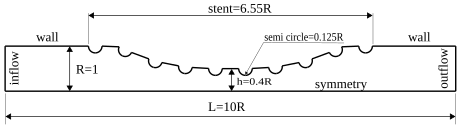
\includegraphics[scale=0.22]{./figure/CurvedStrut.png}\\
     (a) Curved Channel
     \end{center}
     \end{minipage}%
     \begin{minipage}{.45\linewidth}
     \begin{center}
      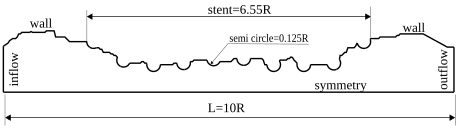
\includegraphics[scale=0.22]{./figure/RealStrut.png}\\
     (b) Real Channel
     \end{center}
     \end{minipage}\\[3mm]
     \end{center}
     \label{coronary artery geo}
     \caption{Non-dimensional domain for the blood flow in coronary artery
     The radius used was $R=1$ and and the lumen length was $L=10R$ as proposed by \cite{wang2017}}
\end{figure}




\subsection{Poiseuille Symmetric Flow} \label{half poiseuille sec}

This section presents the simulation of the \textit{Poiseuille} flow 
in half of the domain. Thus, the free-slip condition is required on 
the axis of symmetry. The Fig. \ref{half poiseuille}  presents schematically 
this flow with the specified axis of symmetry and the expected velocity 
field.

\begin{figure}[H]
\begin{center}
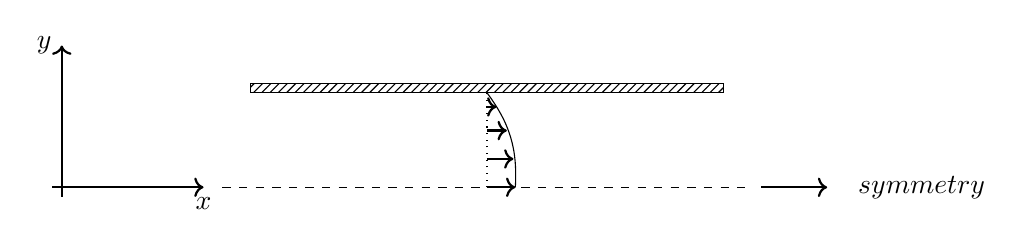
\begin{tikzpicture}[scale=1.2]
 \draw [pattern=north east lines] (0,1) -- (0,1.1) -- (5,1.1) -- (5,1) -- cycle;
 \draw [dashed] (-0.3,0.0) to (5.3,0.0);

 \draw [->,thick] (-2,-0.1)--(-2,1.5) node[left] {$y$};
 \draw [->,thick] (-2.1,0)--(-0.5,0) node[below] {$x$};

 \draw [->,thick] (5.4,0.0)--(6.1,0.0);
 \node [draw=none] at (7.1,0.0) {$symmetry$};
 
 \draw [dotted] (2.5,0.0) to (2.5,1.0);
 \draw  (2.8,0.0) to [bend right=20] (2.5,1.0);
 
 \draw [->,thick] (2.5,0.0) to (2.8,0.0);
 \draw [->,thick] (2.5,0.3) to (2.78,0.3);
 \draw [->,thick] (2.5,0.6) to (2.71,0.6);
 \draw [->,thick] (2.5,0.85) to (2.6,0.85);
\end{tikzpicture}
\end{center}
\label{half poiseuille}
\caption{Half Poiseuille flow}
\end{figure}

\noindent
The velocity profile equation is shown below:

\begin{equation}
 u = u_{max} \big[ 1 - \frac{y^{2}}{L^{2}} \big]
\end{equation}


\medskip
where $u_{max}$ is maximum velocity and its value is 
$u_{max} = 1.5$, $L$ is non-dimensional length 
between the plates and its value is 
$L = 1$
and $y$ is the vertical coordinates and it varies 
between $y = \big[ 0,1 \big]$.
The domain was discretized using a linear triangular mesh
with 3835 nodes and 7299 elements.


\medskip
The Fig. \ref{velocidade half poiseuille}  shows the unsteady velocity profile
when $Re=100$, in addition to the comparison between the 
numerical and analytical solutions in the steady state of
proposed problem. It is possible to observe that the numerical
solution converges to the analytical solution when the flow
becomes steady state.



\begin{figure}[H]
     \centering
     \includegraphics[scale=1]{./figure/half_poiseuille_velocity.pdf}\\
     \medskip
     \label{velocidade half poiseuille}
     \caption{
Unsteady velocity profile when $Re=100$ and the comparison between
the numerical and analytical solution for Half Poiseuille flow.} 
\end{figure}





\subsection{Curved Channel with Stent} \label{canal curvado com stent}

In this section, will be present
the case where the coronary 
artery has atherosclerosis and 
the drug-eluting stent is placed. 
It is modeled by 10 uniformly spaced 
semi-circles. 
The geometry used promotes a smooth reduction of the 
distance between the upper wall and symmetry axis of the channel. 
Due to atherosclerosis, 40\% channel obstruction was considered 
and the domain was discretized using 15875 nodes and 35408 
linear triangular elements. 

\vspace{0.2cm}
\par
The Fig. \ref{velocity evolution curved stent}  shows the unsteady state 
velocity profile in the middle section channel, that is, 
$x=5.0R$. 
As expected, the numerical solution tends to a similar profile to
the Half Poiseuille, as presented in the section \ref{half poiseuille sec} . However, it is possible to observe an inversion of the velocity
field sense at the top of the figure.
This inversion occurs in the region that is
located between the stents strut semi-circles.
It is also possible to observe that the maximum horizontal velocity field 
in curvel channel reaches the $u=3.43$ non-dimensional value, that is, 
more than 3 times the blood velocity in coronary artery
without atherosclerosis and stent strut placed. 
This increase can influence the dynamics of blood flow
and its biological processes and a more detailed analysis
should be performed.

\vspace{1cm}
\begin{figure}[H]
     \centering
     \includegraphics[scale=1]{./figure/vel_CurvedStrut_evol.pdf}\\
     \label{velocity evolution curved stent}
     \caption{
The unsteady state velocity profile in the middle ($x=5.0R$) of the curved channel with drug-eluting stent.}
\end{figure}

\newpage
The Fig. \ref{velocity field curved stent}  presents the evolution in 
time and space of the velocity field for half of the domain
due to the symmetry of the solution. 
The velocity field is represented with non-dimensional values 
where the red color refers to the $u=3.43$ value and the blue color 
$u=0$ value. Conveting to dimensional values, 
we have $u=41.16cm/s$ and $u=0cm/s$ respectively.
As can be seen, the region with the lowest horizontal velocity 
magnitude is found close to the boundary where the no-slip
condition is applied. Whereas, it is increase close to 
the symmetric axis. Moreover, the largest horizontal velocity value
is found in the maximum contraction region.


\vspace{1cm} 
\begin{figure}[H]
     \begin{minipage}{.50\linewidth}
      \centering
      \includegraphics[scale=0.18]{./figure/vel_CurvedStrut1.png}\\
      t = 0.1s
     \end{minipage}%
     \begin{minipage}{.50\linewidth}
      \centering
      \includegraphics[scale=0.18]{./figure/vel_CurvedStrut2.png}\\
      t = 0.5s
     \end{minipage}
     \begin{minipage}{.50\linewidth}
     \medskip
      \centering
      \includegraphics[scale=0.18]{./figure/vel_CurvedStrut3.png}\\
      t = 1.0s
     \end{minipage}%
     \begin{minipage}{.50\linewidth}
     \medskip
      \centering
      \includegraphics[scale=0.18]{./figure/vel_CurvedStrut4.png}\\
      t = 3.0s
     \end{minipage}
     \begin{minipage}{.50\linewidth}
      \centering
      \includegraphics[scale=0.18]{./figure/vel_CurvedStrut5.png}\\
      t = 5.0s
     \end{minipage}%
     \begin{minipage}{.50\linewidth}
      \centering
      \includegraphics[scale=0.18]{./figure/vel_CurvedStrut6.png}\\
      t = 7.0s
     \end{minipage}
     \begin{minipage}{.50\linewidth}
     \medskip
      \centering
      \includegraphics[scale=0.18]{./figure/vel_CurvedStrut7.png}\\
      t = 10.0s
     \end{minipage}%
     \begin{minipage}{.50\linewidth}
     \medskip
      \centering
      \includegraphics[scale=0.18]{./figure/vel_CurvedStrut8.png}\\
      t = 100.0s
     \end{minipage}\\[10pt]
      \centering
      \includegraphics[scale=0.5]{./figure/vel_CurvedStrutScale.png}\\
     \medskip
     \label{velocity field curved stent}
     \caption{
Temporal and spatial evolution of the velocity field for curved channel with
drug-eluting stent.}
\end{figure}


\smallskip
As mentioned by Lucena et al. (2018) \cite{lucena2018}, 
it is estimated that 47\% of the drug is diffused to the 
lumem and it is lost to the bloodstream.
The Fig. \ref{conc field curved stent sc 10}  shows the temporal and spatial evolution 
of the concentration field for the \textit{Schmidt} number equal to $10$.
The concentration field is 
represented with the non-dimensional values where the red color 
represents $100$\% and the blue color represents $0$\% 
of the diffused concentration in the bloodstream. 

\medskip
It is possible to observe in the Fig. \ref{conc field curved stent sc 10}  that
the concentration field
is more dispersed at the end of the curved channel due to
the sense of the blood flow. It is possible that the
drug concentration diffused affects the density and viscosity of the blood
and consequently the Reynolds number. Thefore, the velocity field would
also be affected. However, this influence is not considered in this work.

\begin{figure}[H]
     \begin{minipage}{.50\linewidth}
      \centering
      \includegraphics[scale=0.18]{./figure/conc10_CurvedStrut1.png}\\
      t = 0.1s
     \end{minipage}%
     \begin{minipage}{.50\linewidth}
      \centering
      \includegraphics[scale=0.18]{./figure/conc10_CurvedStrut2.png}\\
      t = 0.5s
     \end{minipage}
     \begin{minipage}{.50\linewidth}
     \medskip
      \centering
      \includegraphics[scale=0.18]{./figure/conc10_CurvedStrut3.png}\\
      t = 1.0s
     \end{minipage}%
     \begin{minipage}{.50\linewidth}
     \medskip
      \centering
      \includegraphics[scale=0.18]{./figure/conc10_CurvedStrut4.png}\\
      t = 3.0s
     \end{minipage}
     \begin{minipage}{.50\linewidth}
      \centering
      \includegraphics[scale=0.18]{./figure/conc10_CurvedStrut5.png}\\
      t = 5.0s
     \end{minipage}%
     \begin{minipage}{.50\linewidth}
      \centering
      \includegraphics[scale=0.18]{./figure/conc10_CurvedStrut6.png}\\
      t = 7.0s
     \end{minipage}
     \begin{minipage}{.50\linewidth}
     \medskip
      \centering
      \includegraphics[scale=0.18]{./figure/conc10_CurvedStrut7.png}\\
      t = 10.0s
     \end{minipage}%
     \begin{minipage}{.50\linewidth}
     \medskip
      \centering
      \includegraphics[scale=0.18]{./figure/conc10_CurvedStrut8.png}\\
      t = 100.0s
     \end{minipage}\\[10pt]
      \centering
      \includegraphics[scale=0.5]{./figure/conc1_CurvedStrutScale.png}\\
     \medskip
     \label{conc field curved stent sc 10}
    \caption{
Temporal and spatial evolution of the concentration fiel for curved channel with drug-eluting stent and $Sc=10$.}
\end{figure}


\subsection{Real Channel with Stent} \label{canal real com stent}

For this case, the numerical simulation is performed for a real 
coronary artery with atherosclerosis whose geometry was obtained 
through an image processing as suggested by Wang et al. (2017) 
\cite{wang2017}. This geometry is particular to each patient 
due to the patient health conditions. As in the previous case, 
the stent strut was modeled by
10 uniformly spaced semi-circles.
The domain was discretized using 11807 nodes and 26426 linear 
triangular elements. 

\medskip
The Fig. \ref{velocity evolution real stent}  shows the unsteady state velocity 
profile in the middle of the real channel, that is,
$x=5.0R$.
Even so, the numerical solution shown a simular
profile to the previous case,
however it is not observed the inversion of the velocity field sense. 
It is also possible to observer that
the maximum non-dimensional value of the velocity field 
reaches $u=3.40$ close to symmetric axis. 
However, this velocity may vary according to the 
coronary artery geometry for each patient.
It compared to the curved channel, the maximum horizontal velocity
had a difference less than $1\%$. Therefore, the curved channel
shown an acceptable approach,
besides this model being simpler to implement
and to perform the numerical simulations than real channel model.

\vspace{1cm}
\begin{figure}[H]
     \centering
     \includegraphics[scale=1]{./figure/vel_RealStrut_evol.pdf}\\
     \label{velocity evolution real stent}
     \caption{
The unsteady state velocity profile in the middle of the real channel with drug-eluting stent.}
\end{figure}

\medskip
The Fig. \ref{velocity field real stent}  presents the evolution in 
time and space of the velocity field for half of the domain. 
The velocity field is represented with non-dimensional values 
where the red color refers to the $u=3.40$ value and the blue color 
$u=0$ value. Conveting to dimensional values, 
we have $u=40.8cm/s$ and $u=0cm/s$ respectively. As in the previous case,
the region with the lowest horizontal velocity magnitue is found close to
the boundary due to the no-slip
condition and the largest horizontal
velocity value is found close to
symmetric axis. For this real channel, is possible to observe that
there is two contraction region where
the velocity field is increased.
However, this coronary artery geometry varies for each patient and its blood dynamics can be changed.


\vspace{1cm} 
\begin{figure}[H]
     \begin{minipage}{.50\linewidth}
      \centering
      \includegraphics[scale=0.18]{./figure/vel_RealStrut1.png}\\
      t = 0.1s
     \end{minipage}%
     \begin{minipage}{.50\linewidth}
      \centering
      \includegraphics[scale=0.18]{./figure/vel_RealStrut2.png}\\
      t = 0.5s
     \end{minipage}
     \begin{minipage}{.50\linewidth}
     \medskip
      \centering
      \includegraphics[scale=0.18]{./figure/vel_RealStrut3.png}\\
      t = 1.0s
     \end{minipage}%
     \begin{minipage}{.50\linewidth}
     \medskip
      \centering
      \includegraphics[scale=0.18]{./figure/vel_RealStrut4.png}\\
      t = 3.0s
     \end{minipage}
     \begin{minipage}{.50\linewidth}
      \centering
      \includegraphics[scale=0.18]{./figure/vel_RealStrut5.png}\\
      t = 5.0s
     \end{minipage}%
     \begin{minipage}{.50\linewidth}
      \centering
      \includegraphics[scale=0.18]{./figure/vel_RealStrut6.png}\\
      t = 7.0s
     \end{minipage}
     \begin{minipage}{.50\linewidth}
     \medskip
      \centering
      \includegraphics[scale=0.18]{./figure/vel_RealStrut7.png}\\
      t = 10.0s
     \end{minipage}%
     \begin{minipage}{.50\linewidth}
     \medskip
      \centering
      \includegraphics[scale=0.18]{./figure/vel_RealStrut8.png}\\
      t = 100.0s
     \end{minipage}\\[10pt]
      \centering
      \includegraphics[scale=0.5]{./figure/vel_RealStrutScale.png}\\
     \medskip
      \label{velocity field real stent}
    \caption{
Temporal and spatial evolution of the velocity field for real channel with
drug-eluting stent.}
\end{figure}


\smallskip
The Fig. \ref{conc field real stent sc 10}  shows the temporal and spatial evolution 
of the concentration field for the \textit{Schmidt} number equal to $10$. 
The concentration field is 
represented with the non-dimensional values where the red color 
represents $100$\% and the blue color represents $0$\% 
of the diffused concentration in the bloodstream. 
It is possible to observe that the concentration field dynamic
is similar than the curved channel, no significant differences
from the previous one Schmidt number.
Only in some regions that the concentration field
become more diffuse as a consequence of the velocity 
field decrease due to irregular geometry close to the
semi-circles of the stents.


\begin{figure}[H]
     \begin{minipage}{.50\linewidth}
      \centering
      \includegraphics[scale=0.18]{./figure/conc10_RealStrut1.png}\\
      t = 0.1s
     \end{minipage}%
     \begin{minipage}{.50\linewidth}
      \centering
      \includegraphics[scale=0.18]{./figure/conc10_RealStrut2.png}\\
      t = 0.5s
     \end{minipage}
     \begin{minipage}{.50\linewidth}
     \medskip
      \centering
      \includegraphics[scale=0.18]{./figure/conc10_RealStrut3.png}\\
      t = 1.0s
     \end{minipage}%
     \begin{minipage}{.50\linewidth}
     \medskip
      \centering
      \includegraphics[scale=0.18]{./figure/conc10_RealStrut4.png}\\
      t = 3.0s
     \end{minipage}
     \begin{minipage}{.50\linewidth}
      \centering
      \includegraphics[scale=0.18]{./figure/conc10_RealStrut5.png}\\
      t = 5.0s
     \end{minipage}%
     \begin{minipage}{.50\linewidth}
      \centering
      \includegraphics[scale=0.18]{./figure/conc10_RealStrut6.png}\\
      t = 7.0s
     \end{minipage}
     \begin{minipage}{.50\linewidth}
     \medskip
      \centering
      \includegraphics[scale=0.18]{./figure/conc10_RealStrut7.png}\\
      t = 10.0s
     \end{minipage}%
     \begin{minipage}{.50\linewidth}
     \medskip
      \centering
      \includegraphics[scale=0.18]{./figure/conc10_RealStrut8.png}\\
      t = 100.0s
     \end{minipage}\\[10pt]
      \centering
      \includegraphics[scale=0.5]{./figure/conc1_RealStrutScale.png}\\
     \medskip
     \label{conc field real stent sc 10}
    \caption{
Temporal and spatial evolution of the concentration fiel for real channel with drug-eluting stent and $Sc=10$.}
\end{figure}




\section{CONCLUSION}
In this work, a numerial code for Navier-Stokes equation according to 
the stream-vorticity formulation with species
transport equation was developed using an ALE-FE approach.
The semi-Lagrangian scheme was used to discretized the material derivative
using first order backward difference scheme and the numerical oscillations
were not seen for moderate to high Schmidt number.

\smallskip
The dynamics of blood flow was shown to a coronary artery with atherosclerosis and
drug-eluting stent placed.
It is possible to observe in the Fig. \ref{conc field curved stent sc 10}  that
the concentration field
is more dispersed at the end of the curved channel due to
the sense of the blood flow. It is possible that the
drug concentration diffused affects the density and viscosity of the blood
and consequently the Reynolds number. Thefore, the velocity field would
also be affected. However, this influence is not considered in this work.




\section{ACKNOWLEDGEMENTS}
The authors thank the 
FAPERJ (Research Support Foundation of the State of Rio de Janeiro)
for its financial support.


\section{REFERENCES} 
\bibliographystyle{abcm}
\renewcommand{\refname}{}
\bibliography{references}

\end{document}



\end{document}
